\documentclass{article} 
\usepackage[left=0.75in,top=0.6in,right=0.75in,bottom=0.6in]{geometry} % Document margins
\usepackage{tabularx}
\usepackage{fancyvrb}
%\usepackage[hidelinks]{hyperref}
\usepackage{graphicx}
\usepackage{float}
\usepackage{fancyhdr}
\usepackage{geometry}
\usepackage{lastpage}
\usepackage{tabu}

\geometry{
  top=1in,            % <-- you want to adjust this
  inner=0.5in,
  outer=0.5in,
  bottom=1in,
  headheight=5ex,       % <-- and this
  headsep=4ex,          % <-- and this
}

\pagestyle{fancy}
\fancyhf{}
\rhead{\Large\textit{Old Dominion University}}
\lhead{\Large\textit{ECE 432: Assignment 4}}
\cfoot{Page \thepage \hspace{1pt} of \pageref{LastPage}}
\renewcommand{\footrulewidth}{1pt}

\begin{document}

%----------------------------------------------------------------------------------------
%		 TITLE PAGE
%----------------------------------------------------------------------------------------

\begin{titlepage}

\vspace*{45 pt}
\begin{center}
\Huge{\bf CS 432/532:  Web Science}\\
\huge{Spring 2017\\}

\vspace{60 pt}
\Huge\underline {Assignment 4}\\

\vspace{10 pt}
\Huge{Michael Micros}\\\

{\Large \bf {Instructor: Michael L. Nelson}}\\

\vspace{230 pt}
{\huge \bf {Old Dominon University}}\\
{\huge \bf {Norfolk, Virginia}}\\

\vspace{10 pt}
\today

\end{center}
\end{titlepage}




%----------------------------------------------------------------------------------------
%		PROBLEM 1
%----------------------------------------------------------------------------------------

\section*{{\underline{\huge {Problem 1:}} Friendship Paradox for Dr. Nelson's Facebook}}
	 As part of the first problem, Dr. Nelson's facebook graphml file was provided. In order to extract the relevant information from this file the ``pygraphml'' library was imported. This library allows the user to parse the .graphml file and extract the nodes, isolating the desired information which in this count was the ``friend\_count" attribute. It was noted that not all of the users had a ``friend\_count" category. The friend count for all the friends was saved into a file and loaded to RStudio where the mean, median and standard deviation were calculated ( performing the calculations in R was slightly more convenient, instead of importing ``numpy" in Python). In the figure below 3 values stand out: 1) Dr. Nelson's friend count in Red, 2) The median in Green, 3) The mean in Yellow. Note that the Friendship Paradox is true, since Dr. Nelson's friend count is well below both the mean and the median.

\begin{figure}[H]
 \centering
 	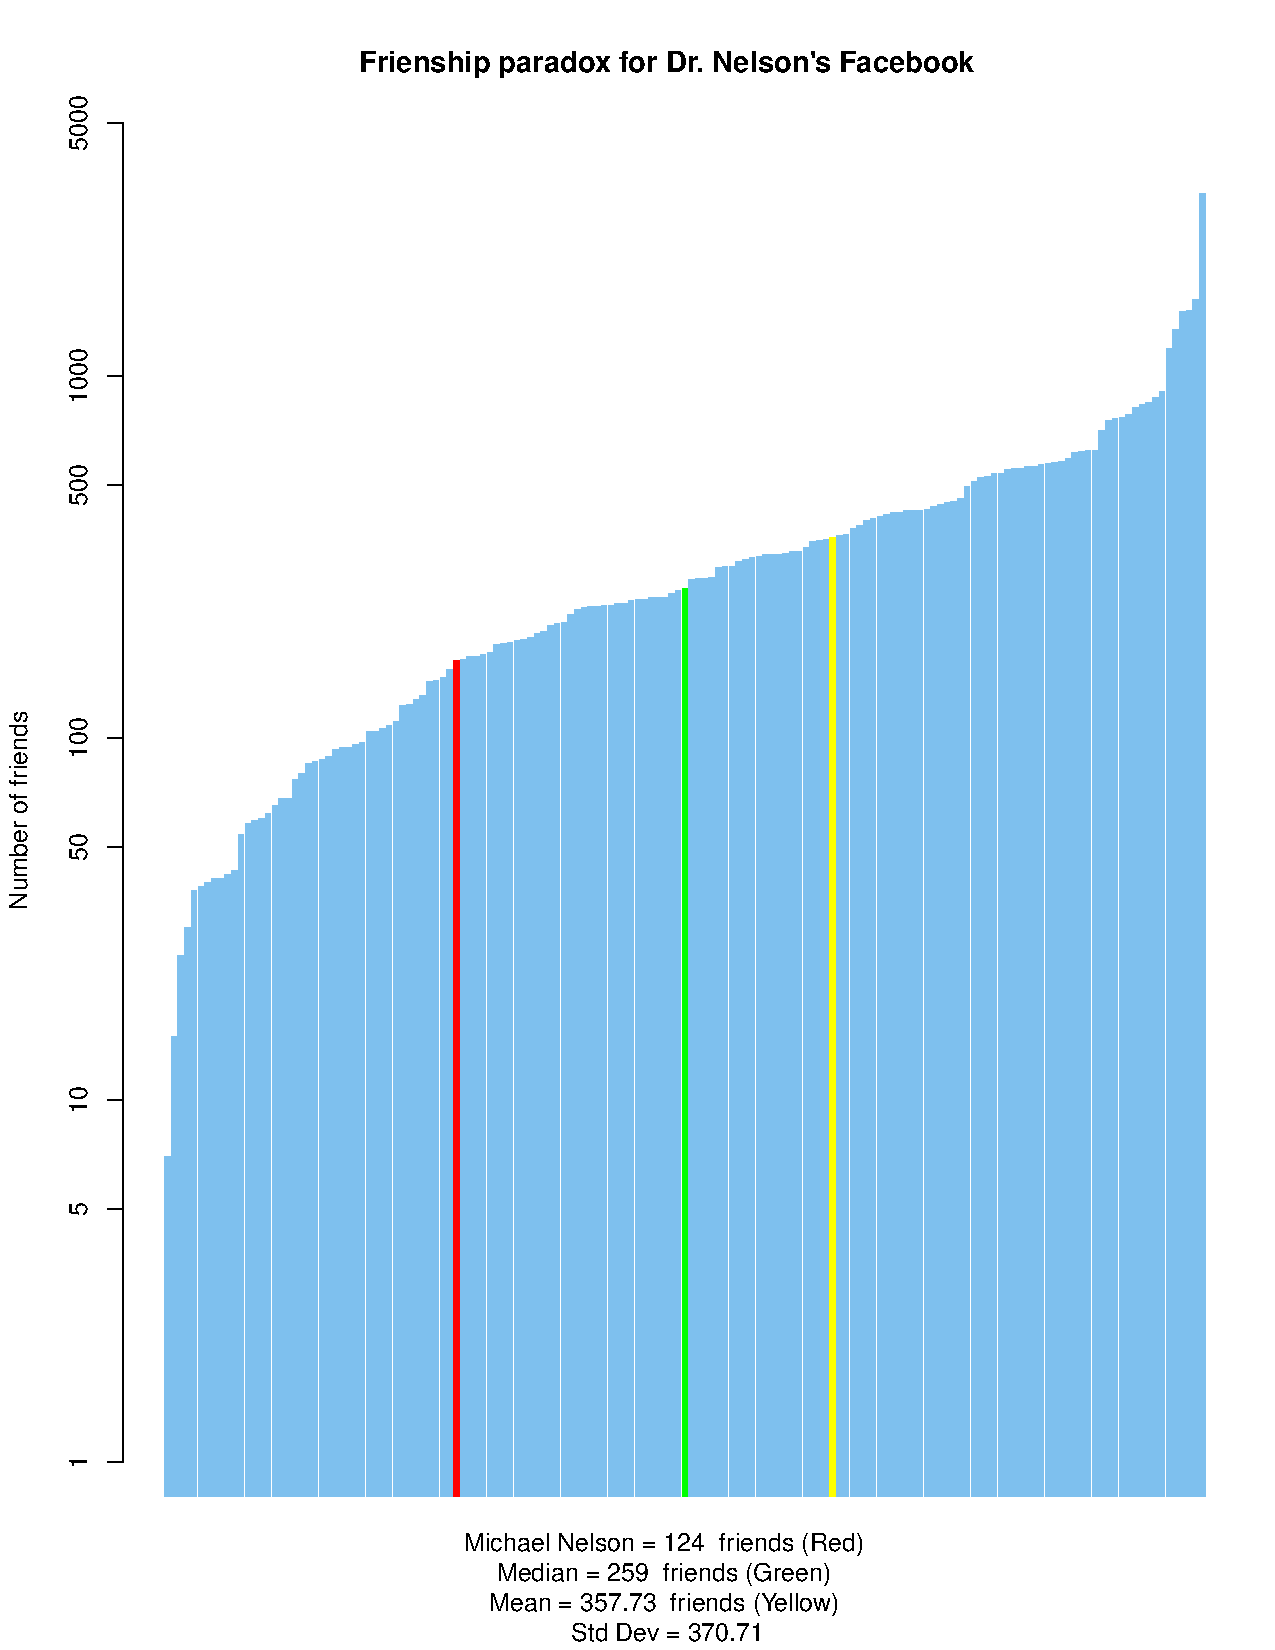
\includegraphics[height=17 cm]{facebook.pdf}
  \caption{Plot of Dr. Nelsons friends VS their friend count}
\end{figure}

\begin{figure}[H]
 \centering
 	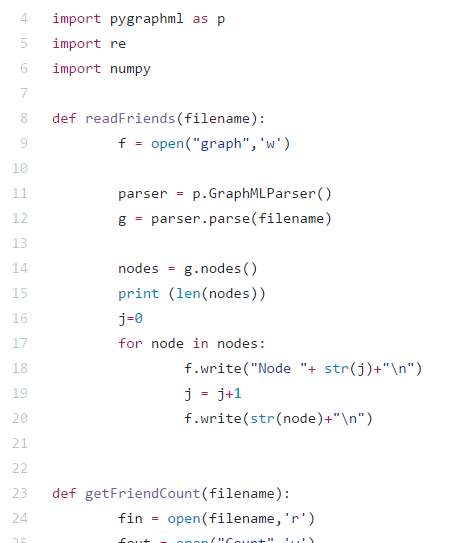
\includegraphics[height=12 cm]{p1code.png}
  \caption{Part of the code in ``p1.py'' that parses the .graphml file and extracts the nodes}
\end{figure}
%----------------------------------------------------------------------------------------
%		PROBLEM 2
%----------------------------------------------------------------------------------------

\newpage
\section*{{\underline{\huge {Problem 2:}} Friendship Paradox for Dr. Nelson's Twitter}}
Similarly to assignment 2, in order to gain access to data on Twitter, we must import tweepy and set up an API. Because I have only 2 followers, Dr. Nelson's twitter was used for this part of the assignment. First, the list of followers is collected and then the ``followers\_count'' is isolated as can be seen in the figure below. Just as in Problem 1, the list was imported into RStudio for  statistical calculations and plotting. We can note that once again the Friendship Paradox hold true, even though Dr. Nelson has more followers than half of his friends (median) 

\begin{figure}[H]
 \centering
 	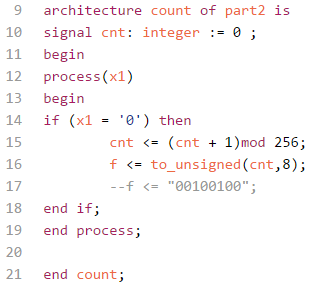
\includegraphics{p2code.png}
  \caption{``p2.py'' Code }
\end{figure}

\begin{figure}[H]
 \centering
 	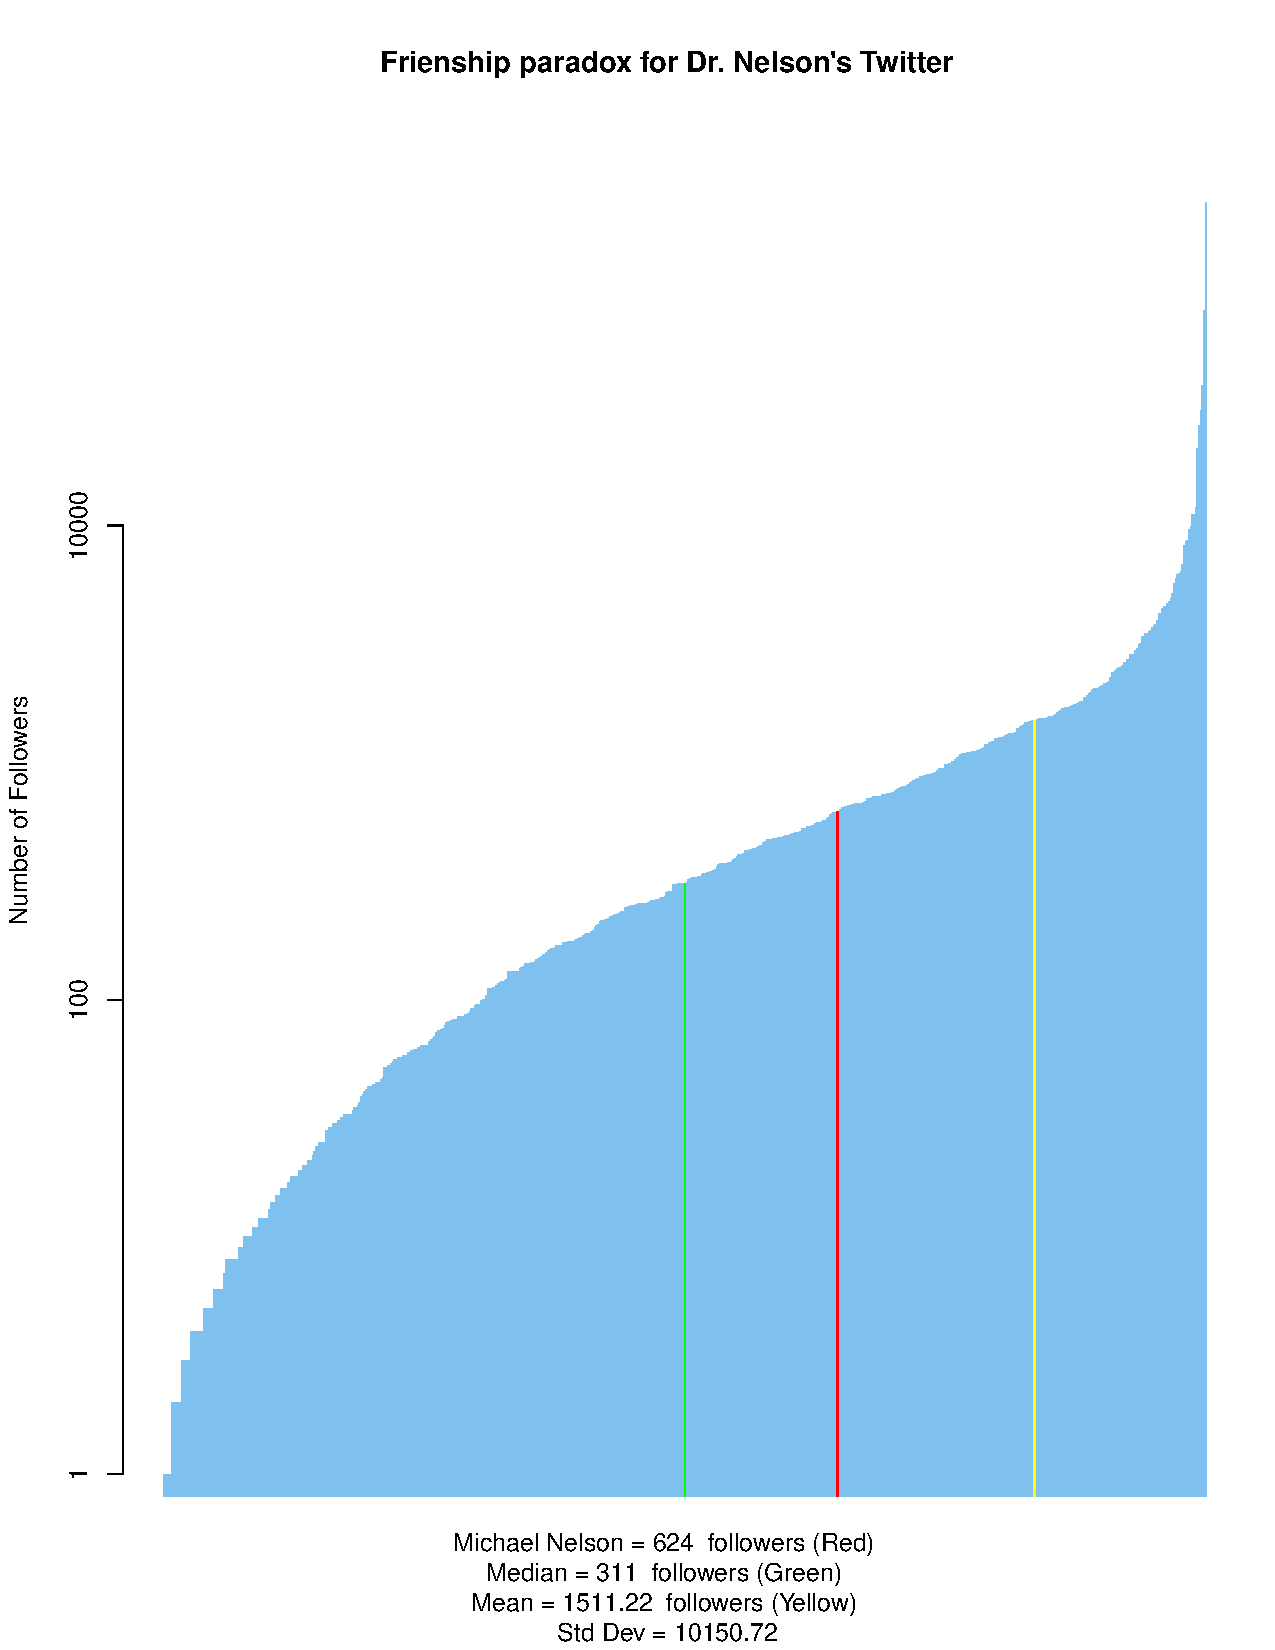
\includegraphics[height = 20 cm]{twitter.pdf}
  \caption{Plot of Dr. Nelsons followers VS their ``followers\_count"}
\end{figure}

\newpage
\section*{{\underline{\huge {Extra Credit:}}}}
I just wanted to let you know that I really appreciate and enjoy your class, and the fact that I have not done any of the extra credit offered in this and previous assignments is the result of terrible time management on my part and a heavy workload.

%----------------------------------------------------------------------------------------
\end{document}
